In this final section, the application that was developed in the course of this
workshop is presented and some additional information like the link to the
project's presentation on hackster.io are provided.

\subsection{User Manual}
The way the user can interact with the application to
ease its shopping experience will be described subsequently.

\subsubsection{Starting SmartCart}
After starting SmartCart, the user will see the starting screen that is shown in
figure \ref{fig:start}. There are already some items added to
the initial shopping list. A user wanting to add additional items, might just
push the plus-button. 

After the user is done with modifying the shopping list, the shopping can
be started by pushing on ``Go shopping''.
The screen that is depicted in figure \ref{fig:initial} is then shown and
the may now start to switch and add items to the cart by performing gestures
with the smartphone.

\begin{figure}[h]
\captionsetup{justification=centering}
\begin{subfigure}{0.475\textwidth} 
\centering 
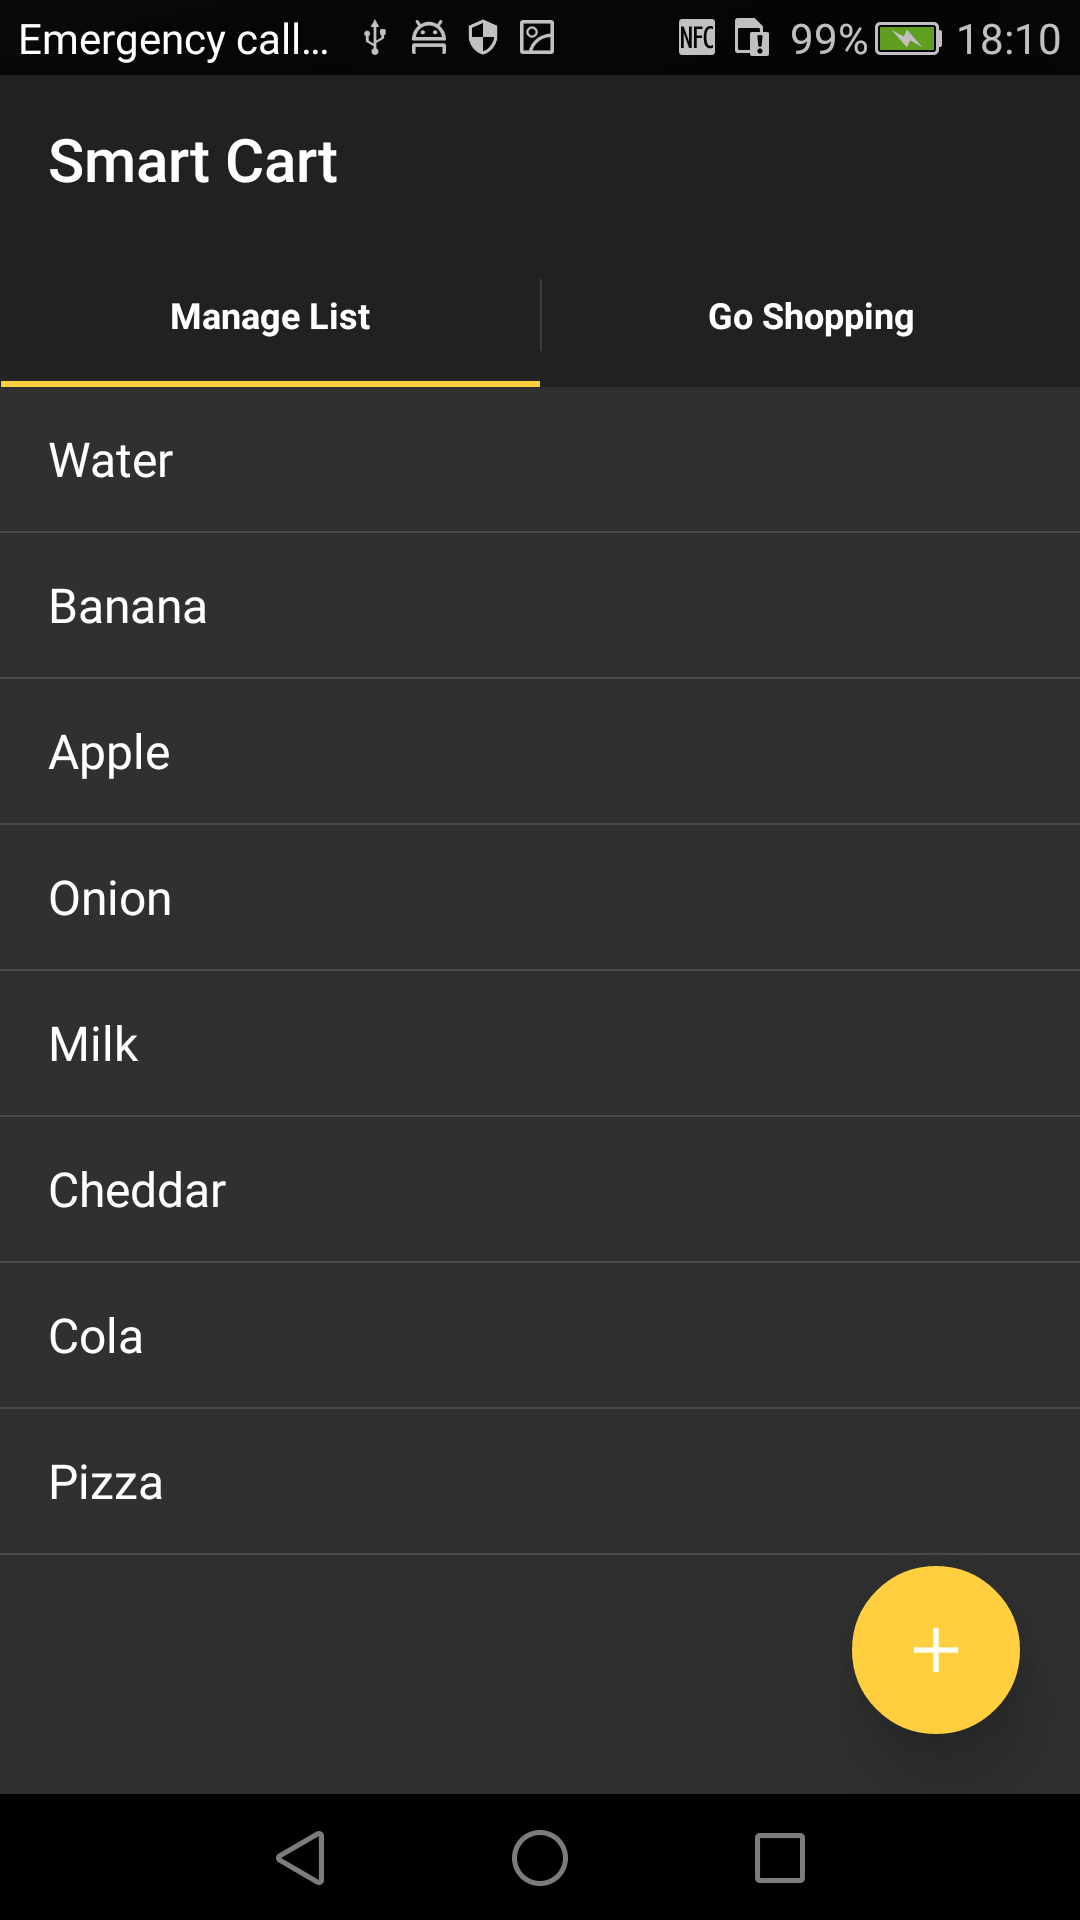
\includegraphics[height= 0.3\textheight]{res/usermanual/startApp.png}
\caption{Start}
\label{fig:start}
\end{subfigure} \hspace{0.05\textwidth}
\begin{subfigure}{0.475\textwidth}
\centering 
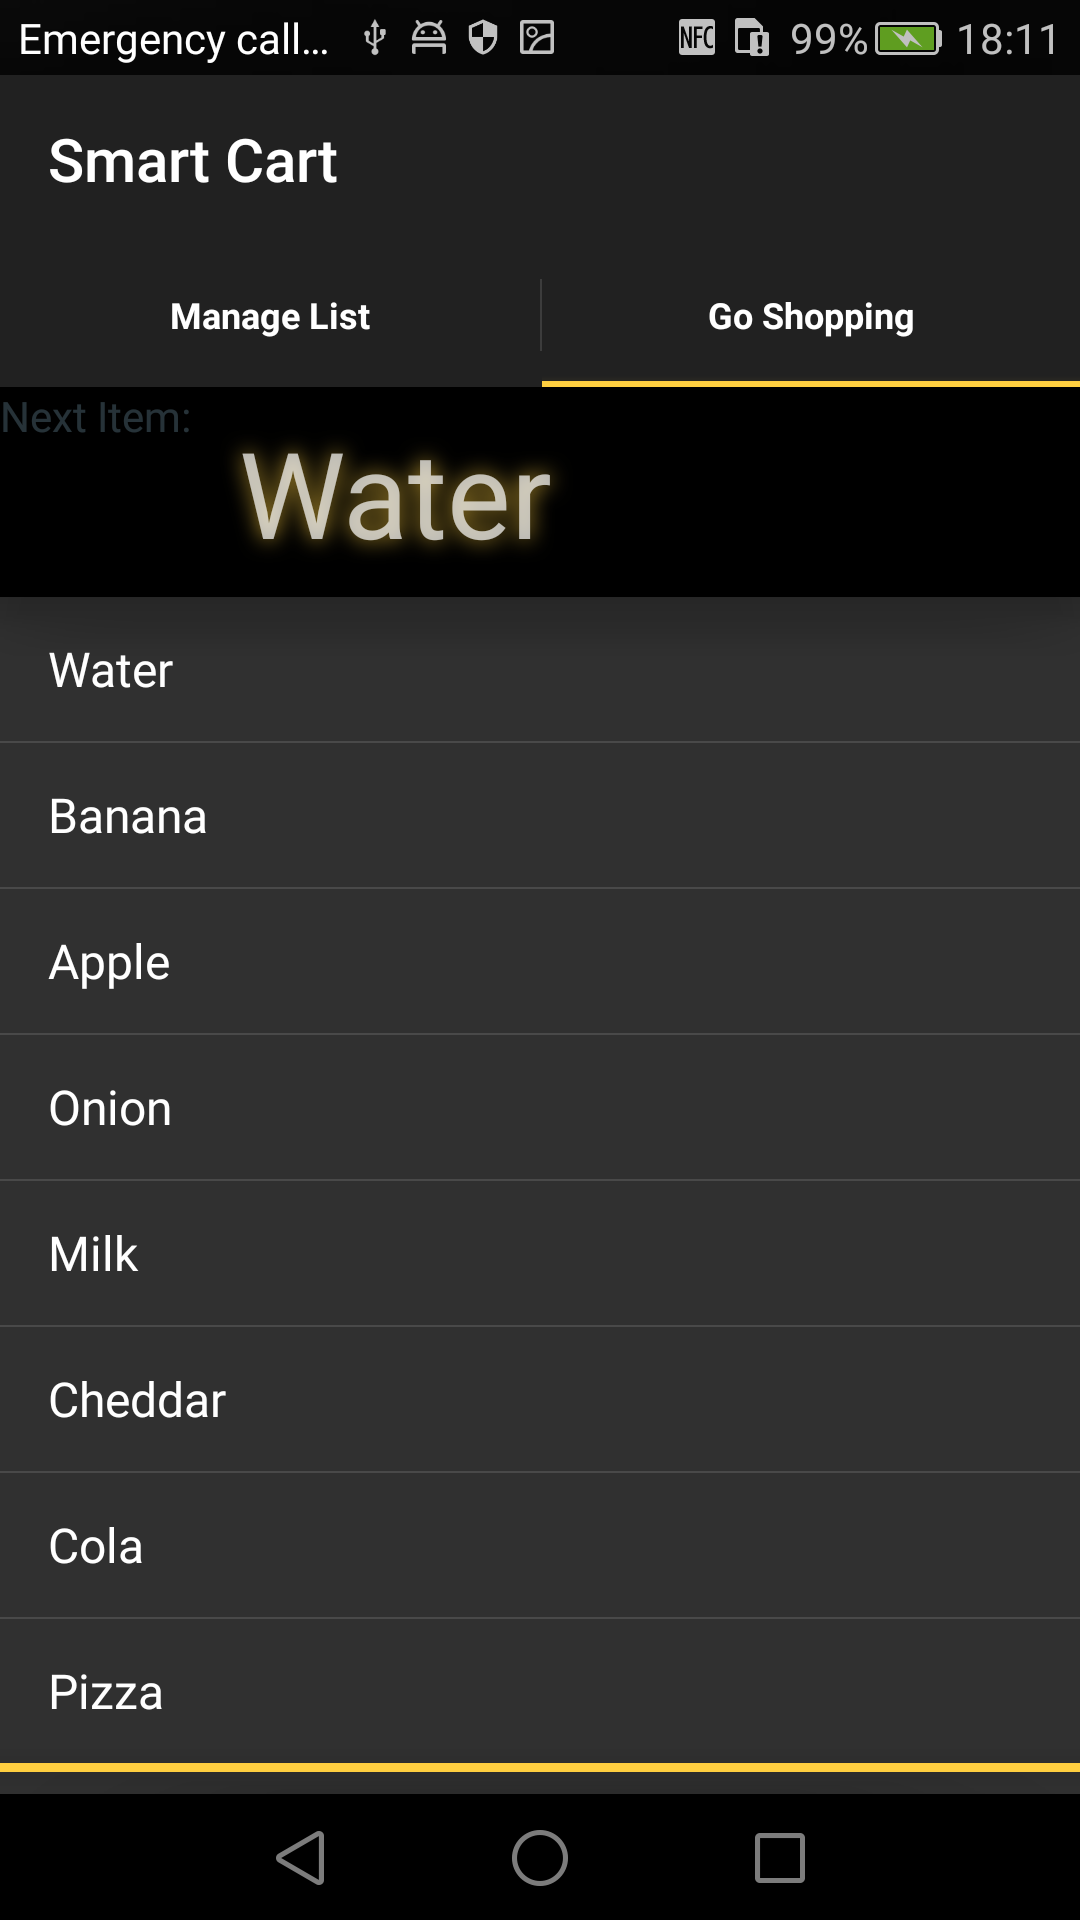
\includegraphics[height= 0.3\textheight]{res/usermanual/initialShoppinglist.png}
\caption{Initial Shoppinglist}
\label{fig:initial}
\end{subfigure}
\caption{Initial State after Starting the App}
\label{fig:initialState}
\end{figure}

\subsubsection{Adding Items to the Cart}
To add the item, that is written in big letters on the top of the list, to the
cart, the user has to perform a circular gesture in the clockwise
direction.
The gesture starts at the bottom of the circle (6 o'clock), moves along the
left-hand side (9 o'clock), the top (12 o'clock) and back to the starting point
(via 3 o'clock). The item that is checked will be moved to the bottom of your list and will be written in
crossed out letters (see figure \ref{fig:firstItemChecked}). The app also
provides its user feedback, if a circle could be recognized and the item could
be added to the cart (see figure \ref{fig:feedbackCircle}).

\begin{figure}[h]
\captionsetup{justification=centering}
\begin{subfigure}{0.475\textwidth} 
\centering 
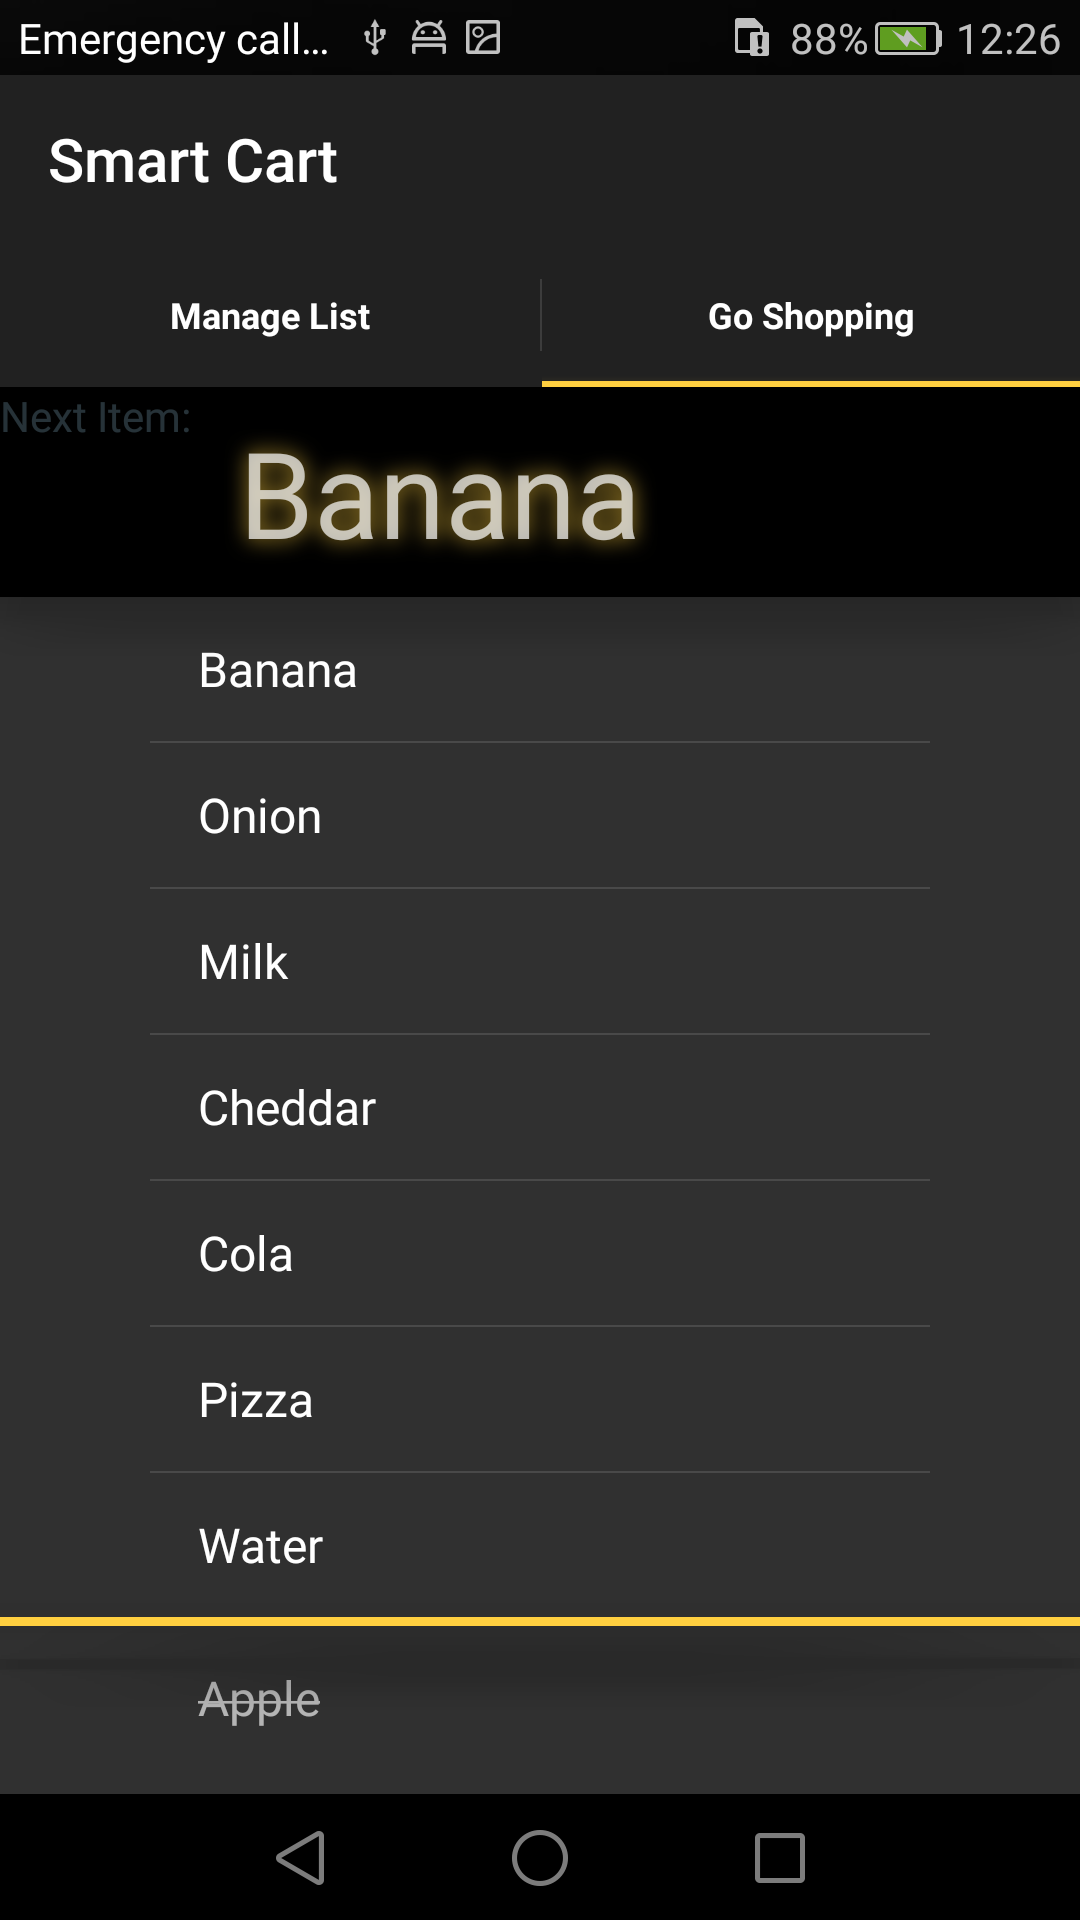
\includegraphics[height= 0.3\textheight]{res/usermanual/firstItemChecked.png}
\caption{First Item Checked Off}
\label{fig:firstItemChecked}
\end{subfigure} \hspace{0.05\textwidth}
\begin{subfigure}{0.475\textwidth}
\centering 
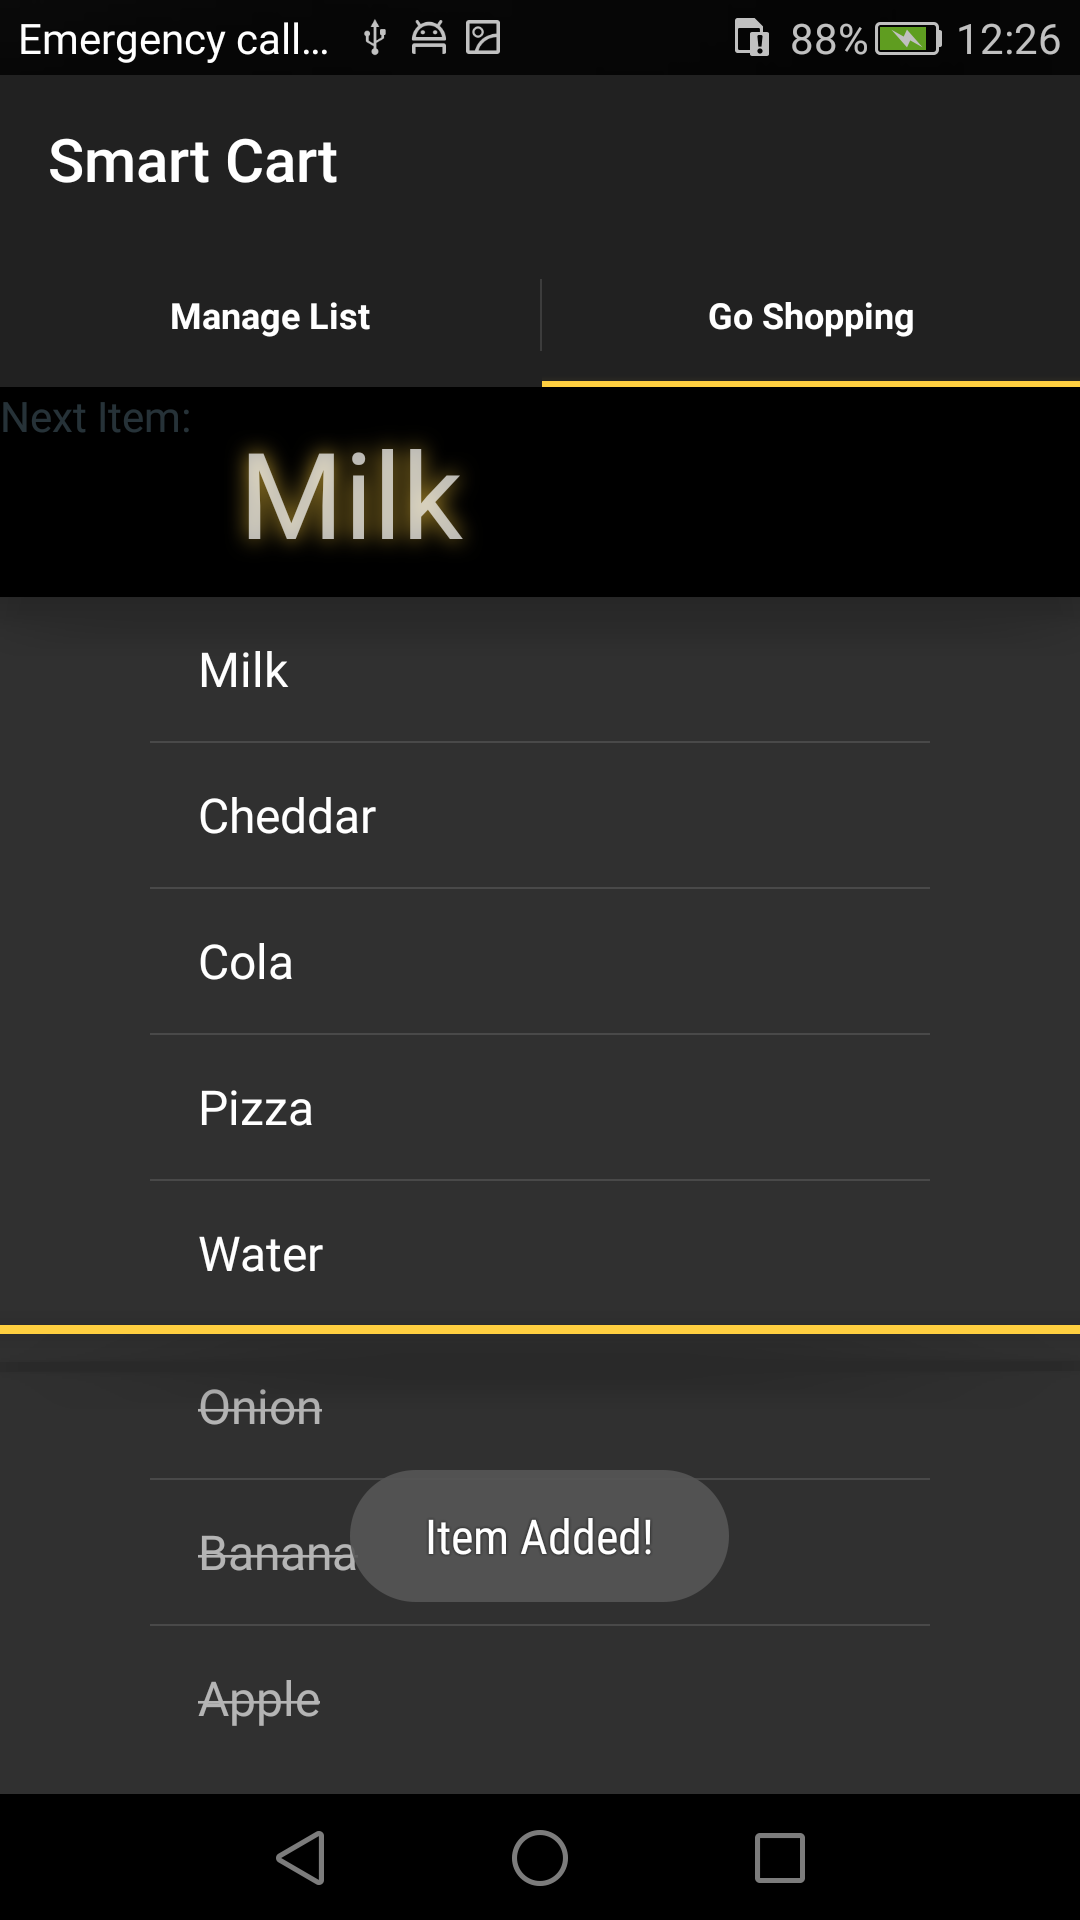
\includegraphics[height= 0.3\textheight]{res/usermanual/circleRecognized.png}
\caption{Feedback Circle Recognized}
\label{fig:feedbackCircle}
\end{subfigure}
\caption{Check Off Items}
\label{fig:checkItems}
\end{figure}

\subsubsection{Switching Items on the List}
If a user wants to add an item to the cart that is not on the top of the list,
he is able to switch the list by performing an circular gesture in the
counter-clockwise direction. The gesture is again started on the bottom of the
circle. Analogous to the case of adding an item to the cart, the SmartCart
application provides feedback to its user about the successful switching of the
list (see figures \ref{fig:beforeSwitching} and \ref{fig:afterSwitching}).

\begin{figure}[h]
\captionsetup{justification=centering}
\begin{subfigure}{0.475\textwidth}
\centering 
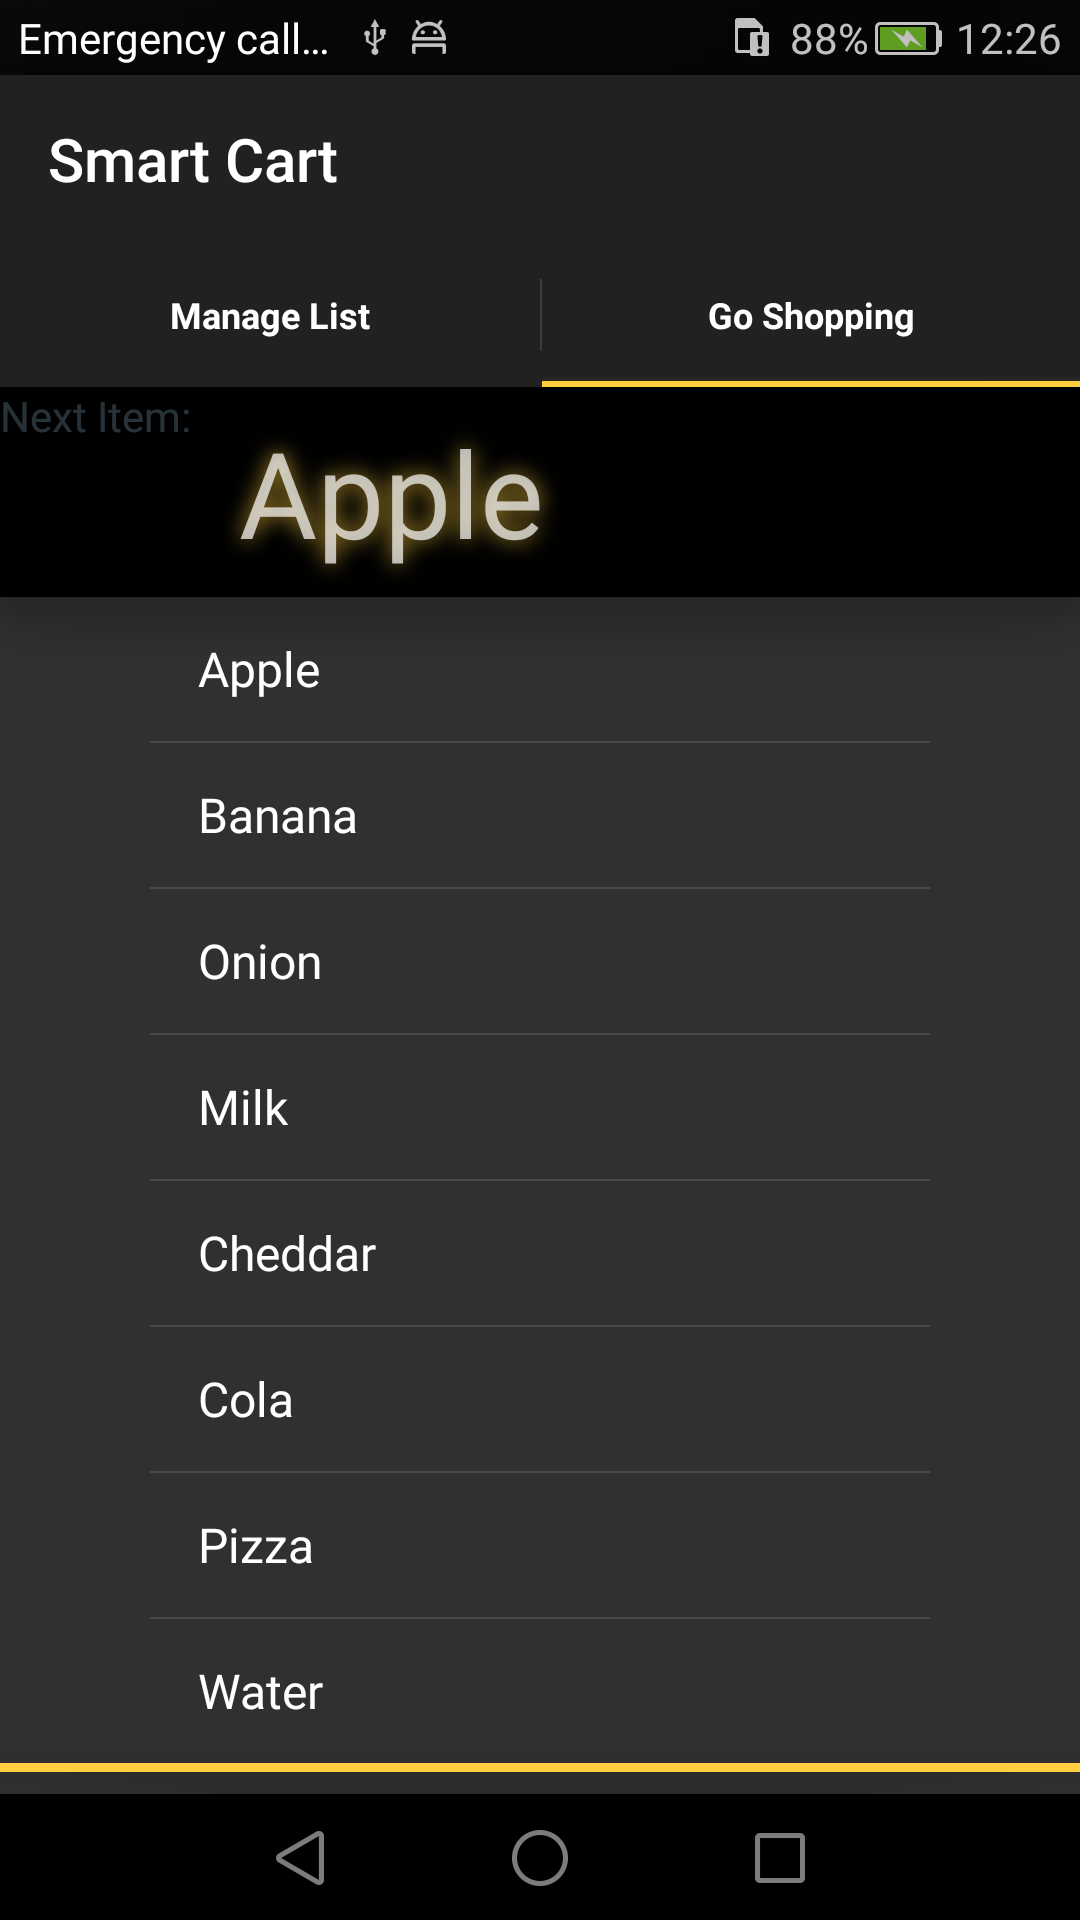
\includegraphics[height= 0.3\textheight]{res/usermanual/notswitched.png}
\caption{Shoppinglist before Switching}
\label{fig:beforeSwitching}
\end{subfigure} \hspace{0.05\textwidth}
\begin{subfigure}{0.475\textwidth}
\centering
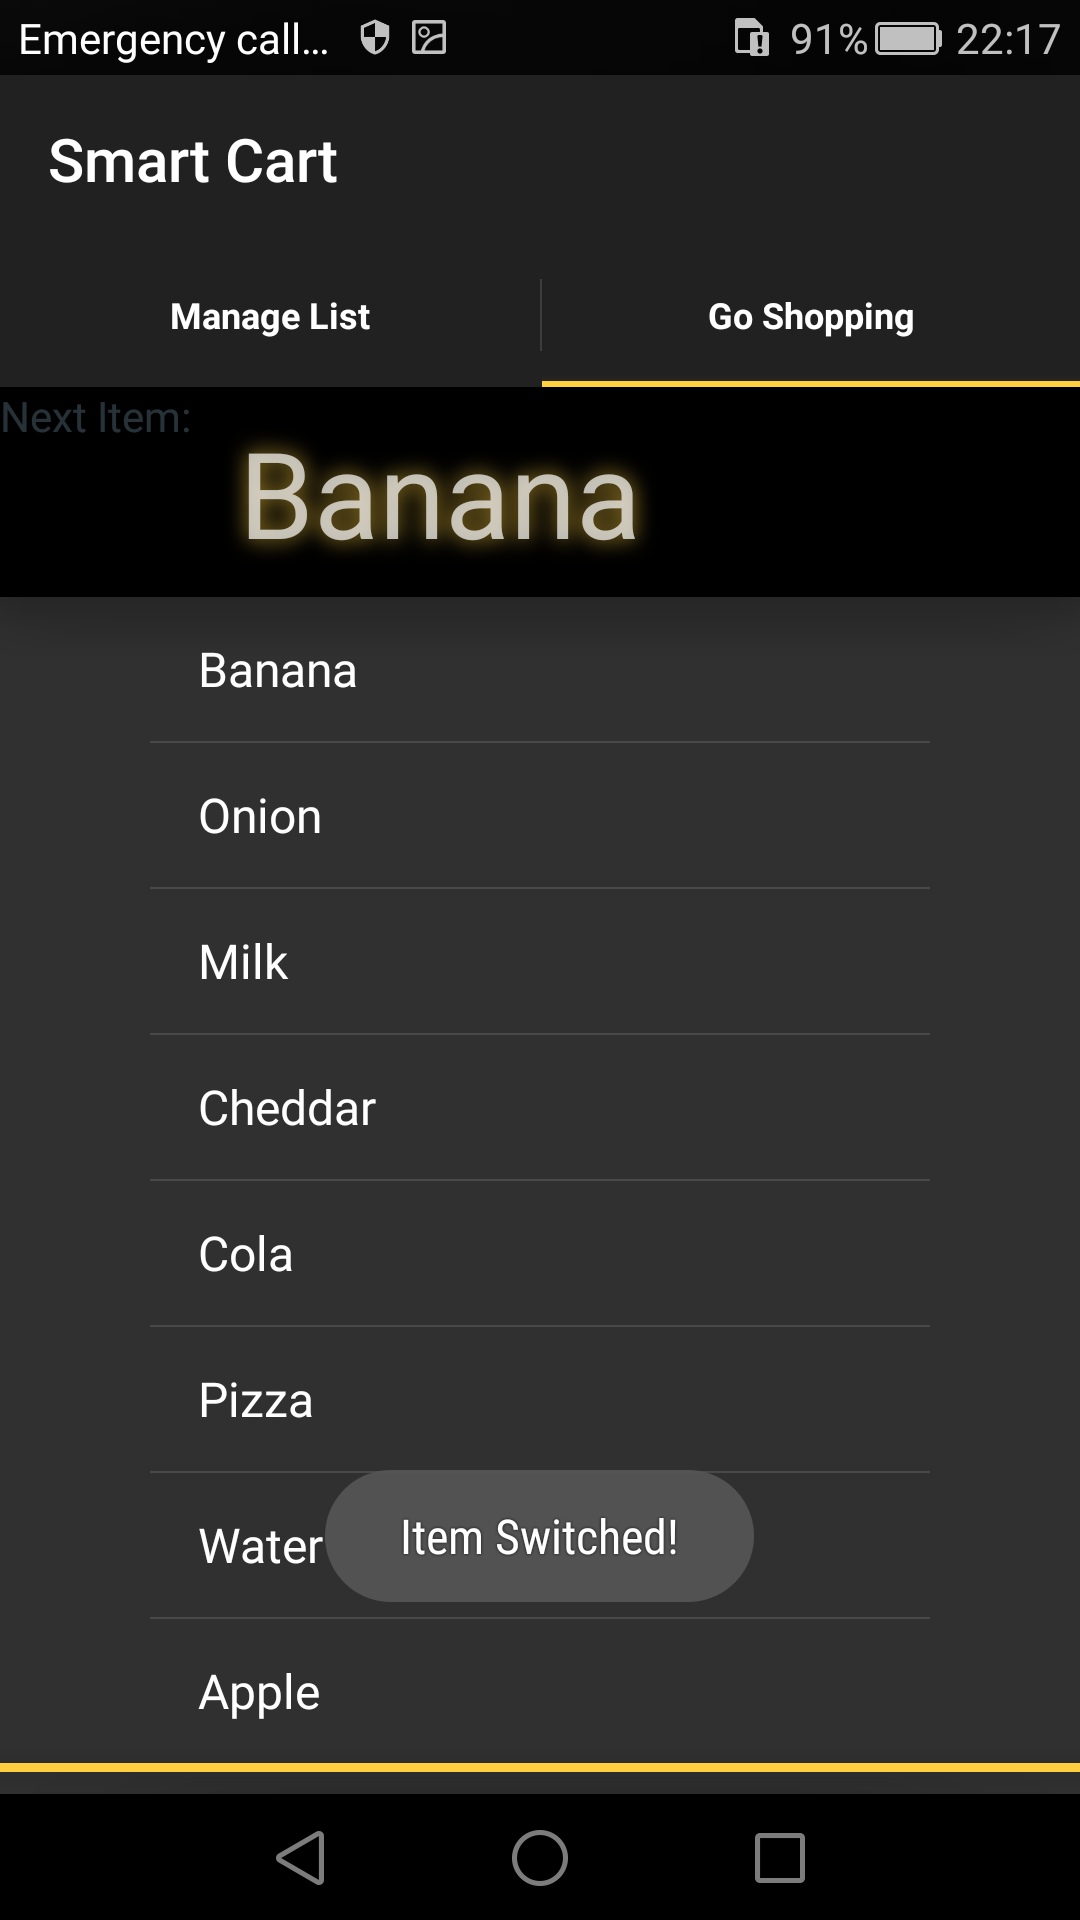
\includegraphics[height= 0.3\textheight]{res/usermanual/switched.png}
\caption{Shoppinglist after Switching}
\label{fig:afterSwitching}
\end{subfigure}
\caption{Switch Items}
\label{fig:checkItems}
\end{figure}

%\FloatBarrier
\subsection{Additional Information}
The project SmartCart was published to hackster.io including a video that
presents the working gesture recognition independent of the smartphone's
orientation. The links to the publications as well as the
user credentials are listed in table \ref{tab:linksCredentials}. The other
resources that were offered in the workshop remained unchanged and are therefore
not listed in the table.

\begin{table}
\centering
\captionsetup{justification=centering}
\footnotesize
\begin{tabular}{p{0.2\textwidth}p{0.35\textwidth}p{0.35\textwidth}}
Resource & Credentials & Link \\
\hline
hackster.io & User: dsce.team.b@gmail.com \newline 
Pass: TWASoEQL &
\url{https://www.hackster.io/dcse-team-b/smart-cart-09155f} \\
youtube.com & User: dsce.team.b@gmail.com \newline 
Pass: TWASoEQL &
\url{https://www.youtube.com/channel/UCpFJqv0PWW_oIS3bQz22KmA} \\
\end{tabular}
\caption{Links and Credentials to/for additional Resources}
\label{tab:linksCredentials}
\end{table}